\documentclass[platex,a4paper,12pt,dvipdfmx]{beamer}
\usetheme{default}
\usepackage{tikz}
\newcommand{\hello}[2]{%
  \node (hi) at (#1,#2) {hello};
}

\begin{document}
\begin{frame}{}
  \begin{tikzpicture}
    \draw[help lines] (-5,-5) grid (5,5);
    \only<1>{\hello{1}{1}}
    \only<2>{\hello{1}{2}}
    \only<3>{\hello{1}{3}}
    \only<4>{\hello{1}{4}}
  \end{tikzpicture}
\end{frame}
\end{document}
